\documentclass{article}
\usepackage{graphicx}
\usepackage{hyperref}
\usepackage{tex4ebook}
\usepackage{ifpdf}
\usepackage{float}
\usepackage{titlesec}
\usepackage{listings}
\usepackage{xcolor}
\usepackage{tikz-timing}[2009/12/09]
\usepackage{variables}
\usepackage{movie15}
\usetikztiminglibrary[new={char=Q,reset char=R}]{counters}

\usepackage{movie15}
\titleformat{\section}[block]{\normalfont\Large\bfseries\raggedright}{\thesection}{1em}{}
\titlespacing*{\section}{0pt}{\baselineskip}{\baselineskip}

\titleformat{\subsection}
  {\normalfont\large\bfseries\raggedright}{\thesubsection}{1em}{}
  [\vspace{1ex}]

\titlespacing*{\subsection}{0pt}{\baselineskip}{\baselineskip}

\titleformat{\subsubsection}
  {\normalfont\normalsize\bfseries\raggedright}{\thesubsubsection}{1em}{}
\titlespacing*{\subsubsection}{0pt}{\baselineskip}{\baselineskip}

\lstset{
  basicstyle=\ttfamily,
  escapeinside=||
}

\setlength{\parskip}{\baselineskip}%
\title{
  
\includegraphics[width=5cm]{Images/Logo.png}\\
  \normalsize Department of Electrical and Computer Engineering\\
  ENEL 453: Digital System Design
}

\date{\semester}

\makeatletter
\renewcommand{\maketitle}{%
  \begin{center}
    {\@title}
    \vspace{1cm} % Space between title and date, adjust as needed
    {\@date}
  \end{center}
}
\makeatother

\begin{document}
\centering

\maketitle
\large Lab 2: Pulse Width Modulation (PWM) and Clock Dividers  \\
Instruction Manual

\raggedright
\normalsize
\section{Overview}

\normalsize
\ifdefined\devinisteaching
ENEL 453 was one of my favorite courses when I took it during my undergrad. It helped inspire me towards pursuing VLSI as a field, and gained me a substantial leg up when it came to designing FPGA based systems. The reason it was as effective as it was is because I played relentlessly with the code, improving both my test benches and my designs. I encourage you to do the same, play with your designs and go beyond what the labs ask of you, I assure you it is the best way to do well in this course. 
\else
 ENEL 453 is a crucial course that can shape your understanding and enthusiasm for VLSI and FPGA-based systems. The effectiveness of this course comes from deeply engaging with the code, refining test benches, and pushing the boundaries of the lab requirements. Engaging in this manner is highly recommended for succeeding in this course.
\fi
\bigskip

\ifdefined\devinisteaching
A word of warning to students who scoff at test benches. By the end of this course your synthesis times for your FPGA may end up exceeding 1 hour. Effective test benches are the only way to complete your labs in a reasonable length of time. If you go further you may end up with synthesis times taking days to complete. Learn to make quality test benches early, and you'll save more time in the long run. 
\else
A word of warning to students who scoff at test benches. By the end of this course your synthesis times for your FPGA may end up exceeding 1 hour. Effective test benches are the only way to complete your labs in a reasonable length of time. If you go further you may end up with synthesis times taking days to complete. Learn to make quality test benches early, and you'll save more time in the long run. 
\fi
\bigskip

\ifdefined\devinisteaching
I am happy to say we are moving to one of my personal favorite FPGA boards. The Basys3 by digilent, a nifty little board with lots 
of peripherals, and a surprisingly powerful Artix 7 FPGA. The manual for the board is available here: \url{\basys3manual}. 
\else
  This course will use the Basys3 by Digilent, an excellent FPGA board that comes with a variety of peripherals and features a powerful Artix 7 FPGA. The manual for the board is available here: \url{\basys3manual}.
\fi

\section{Before You Begin}

    \subsection{Grading}
\vspace{0.5cm}
\\
\textbf{
This lab is worth \laboneisworth{} of your term grade and broken up as:
}
\begin{itemize}
    \item Simulations, Code, and Video Explanation: \laboneisworth
\end{itemize}
\textbf{*There will be an in-lab demonstration/ oral-examination for Lab 4.}
    \subsection{Instructions}
\begin{itemize}
    \item Read through the entire lab manual before beginning on the programming
    \item \textbf{Students are working independently! All boards must be returned at the end of each lab session!}
    \item Backup your projects!
    \item Lab 2 you are only graded on your online submission, nothing in the submission needs to relate to the board.
    \item Submissions should include all of your source files and test bench files, alongside a video explaining them. 
    \item Lab 2 Simulations are due \labTwoSimsDue{}.
    
\end{itemize}

\section{PWM Explained}
PWM Standards for Pulse Width Modulation. This means that the duty cycle of a square wave is being changed over time, this can be simply to dimm an led or for exciting reasons such as communicating information.\\ 
\vspace{0.5cm}
\begin{tikztimingtable}
PWM Signal 0\% Duty Cycle  & LLLLLL \\
PWM Signal 25\% Duty Cycle & LHLLLH \\
PWM Signal 50\% Duty Cycle & LHHLLH \\
PWM Signal 75\% Duty Cycle & LHHHLH \\
PWM Signal 100\% Duty Cycle & HHHHHH \\
  % \extracode
  % \draw (0,0) circle(0.2pt); % Origin Dot
  % \begin{pgfonlayer}{background}
  %   \vertlines[help lines] {0.5,4.5}
  % \end{pgfonlayer}
\end{tikztimingtable}

\vspace{0.5cm}

Here the duty cycle is changing between 4 different states where 0\% represents the output being fully off, and 100\% represents the output being fully on, and the duty cycles in-between represent being on for a different percentage of the time. The easiest way to create this sort of PWM behavior is to have a counter which increments after each clock cycle until hitting a maximum value and resetting. The duty cycle is set by a number, the output is then 1 while the number is less than or equal to it, and zero when it is above it. 

\section{Clock Divider Explained}
Clock Dividers are a useful basic circuit within digital logic. The Artix 7 FPGA on board the Basys 3 has a PLL which can be used to generate various clock frequencies, in theory these frequencies can be up to 1.6 GHz. However, practically speaking you will be limited by the Basys 3's on board oscillator (100Mhz) as well as the speeds of the logic on board the FPGA. For this course we will ignore the PLL and use the on-board clock alongside the digital logic to generate the additional clocks that we need.\\
\vspace{0.5cm}
In this lab you will need to divide the input 100MHz clock down to produce a roughly 20Hz clock. To do this you will need a clock divider of ~5000000.\\ 
\vspace{0.5cm}
Clock Dividers are essentially simple counters and function in a similar manner to PWM Modules. The goal is to count up and change the output from 1 to 0 at the appropriate time so the output is a slower clock which matches the desired speed. If the division is a power of two, this can literally just be a the counter at a specific bit. 

\vspace{0.5cm}
\begin{tikztimingtable}
\raggedright
  CLK & LHLHLHLHLHLHLHLHLHLHLHLHLHLH \\
  Counter [0]  & LHHLLHHLLHHLLHHLLHHLLHHLLHHL \\
  Counter [1]  & LLLHHHHLLLLHHHHLLLLHHHHLLLLH \\
  Counter [2]  & LLLLLLLHHHHHHHHLLLLLLLLHHHHH \\
  % \extracode
  % \draw (0,0) circle(0.2pt); % Origin Dot
  % \begin{pgfonlayer}{background}
  %   \vertlines[help lines] {0.5,4.5}
  % \end{pgfonlayer}
\end{tikztimingtable}
\vspace{0.5cm}

If you are noticing a similarity to PWM Modules this is good because a PWM module can be used as a clock divider when configured appropriately. This is a great case where carefully written code can allow you to save a substantial amount of time. 
\section{Provided Design}
In this lab you are being provided with a half functional design. You can choose to create your own versions of these modules if you would like a challenge; however, if you choose to go this route you must verify your versions to ensure that they function correctly.

You are provided with the following modules:
\begin{itemize}
    \item \textit{doubledabble.sv}, This contains a SystemVerilog implementation of the double dabble algorithm which will convert the input binary number to a binary coded decimal representation. This is required for driving the 7 segment displays. 
    
    \item \textit{debounce.sv}, This contains a SystemVerilog implementation of button debouncer. This compensates for buttons mechanical properties that results in them repeatedly connecting and disconnecting when pressed. Essentially it acts as a delay to prevent the repeated bounces from registering.

    \item \textit{debounce\_wrapper.sv}, This module contains multiple instantiations of the debounce module. It is intended to keep the top level of the design clean by collecting together multiple near identical instantiations of the debounce module. 
    
    \item \textit{sevenseg4ddriver.sv}, this module handles the timing between the four segments of the display on the Basys3. The module takes 4 seven segment inputs along with the system clock and reset, it then drives the seven cathodes and four anodes of the different digits. This was provided because the timing for this component is difficult to verify without a physical board as the FPGA can switch the pins faster than the external driver transistors can switch resulting in the display not functioning correctly.
    
    \item \textit{segment\_mux.sv}, a simple state machine which handles the multiplexing of the different digits of the second segment display. This module is contained inside the \textit{sevenseg4ddriver.sv} module.
    
    \item \textit{pwm\_module.sv} this is the same PWM module as was used in Lab 2. Here it is used inside the \textit{sevenseg4ddriver.sv} module to produce a slower clock for multiplexing the led segments. 
    
    \item \textit{display\_driver.sv} this module integrates the bcd to binary, double dabble, and display multiplexer units into a single cell to keep the higher level cells concise. It takes a minute and second value from the timer module and outputs the correct seven segment anode and cathode values to drive the display.
    
    \item \textit{bcd\_binary.sv}, this module takes the 4 bit binary coded decimal and converts it into 7 segment values. This module is contained within the display driver unit. 
    
    \item \textit{timer.sv}, this module handles the logic of the timer, recieving input from the debounced buttons and providing an output to the display driver. 
    
    \item \textit{time\_counter.sv}, this module handles increment and decrement minutes and seconds. It is used inside the timer module. \textit{I'd recommend reusing this module to produce the stop watch functionality}.
    
    \item \textit{blinking\_binary.sv}, this module takes the blink signal and the 1Hz clock to generate a blinking effect on the display.

    \item \textit{clock\_divider.sv} this module produces a clock divider to generate a 1Hz and 1KHz clock for use within the other modules.
    
    
\end{itemize}
\section{Required Modifications}
For this lab we want you to create a wave effect across the 16 LEDs on the Basys 3 board. The idea is to make the LEDs increase and decrease in brightness with some form of pattern. This will require modifying the top level to instantiate additional copies of the PWM module to drive the other LEDs and the creation of a slow clock to cycle the duty values for creating the effect. 

\raggedright

\subsection{Python Test bench Tool}
To make life easier when testing your design we have put together a testing tool to visualize the light levels of the LEDs based on the simulation outputs. An example text file has been produced by running the provided top-level test bench. The code for the python script has been provided, and anyone wanting to run it can. Ensure the file is in the same directory as the \textit{leds.txt} and ensure that you have the opencv libraries installed. You can also go to \url{\ledvisualzationurl}. This server should be available to anyone connected to the U of C network, either directly or through the U of C VPN. If the server goes down, send an email to \labInstructorEmail and I will bring it back up as soon as possible. 
\begin{verbatim}
function void print_leds_to_file(input bit [15:0] LEDS, input integer file_descriptor);
    integer i;
    string led_values;

    // Check if the file is open
    if (file_descriptor == 0) begin
        $display("Error: File is not open!");
        return;
    end

    // Initialize the led_values string
    led_values = "";
    // Iterate through the LEDS array and append the binary values to the led_values string
    for (i = 0; i < 16; i++) begin
        led_values = {led_values, $sformatf("%b", LEDS[i])};
    end
    $timeformat(-3,10,"");
    $fwrite(file_descriptor, "%0t %s\n", $realtime, led_values);
    
endfunction

always@(led) begin
    $display("led = %b", led);
    print_leds_to_file({led,15'b000000000000000}, file_descriptor);
end

  initial begin   
    file_descriptor = $fopen("leds.txt", "w");
    // ... The rest of your testbench
    // Close the output file
     $fclose(file_descriptor);
    // Finish the simulation
    $finish;
  end
\end{verbatim}

\normalsize
The above code is present in the top level test bench file and is responsible for producing the \textit{leds.txt} which contains the printed LED values alongside the time of that value. Proceed to the led visualization url and use the file to see an approximation of how the leds will appear. 

\begin{figure}[H]
    \centering
    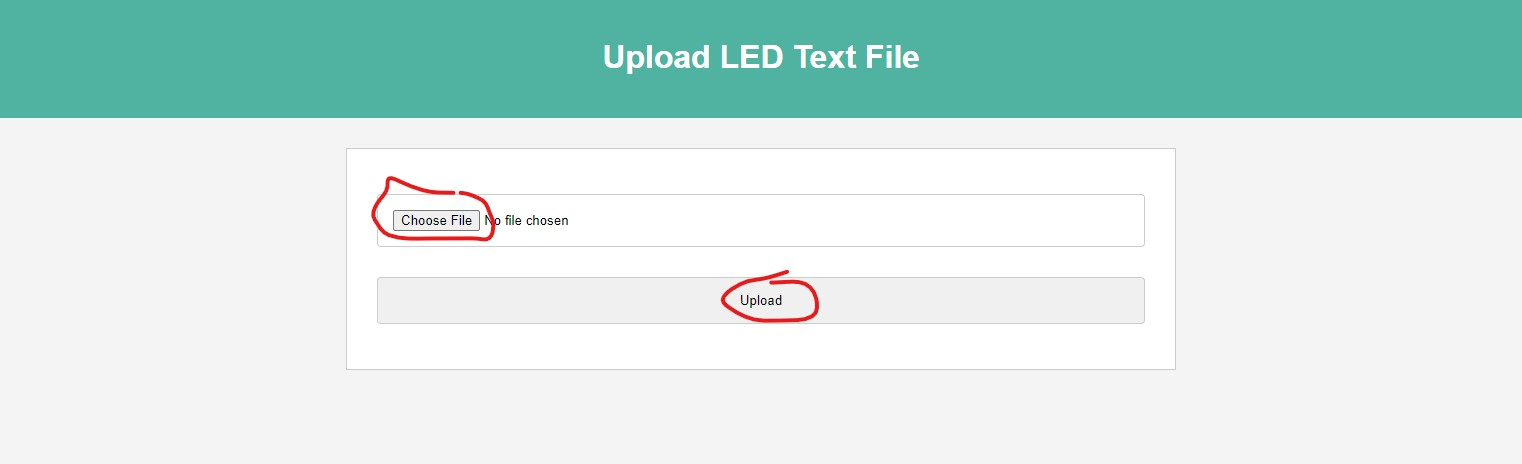
\includegraphics[width=9cm]{Images/ProvidedPWM/LED_VisualizationTool.jpg}
    \caption{LED Visualization Tool}
    \label{fig:enter-label}
\end{figure}
The visualization tool is fairly simple. Click upload file and select the leds.txt file which was created when you ran the simulation. Then press the upload button. The upload will run, and a short video file will be returned.\textit{Generating the video file can take up to 5 minutes for periods of roughly 1 second!} The video will look somewhat like the following.
\begin{figure}[H]
    \centering
    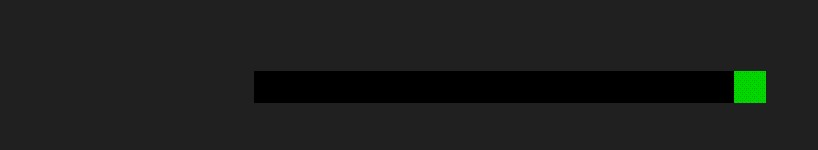
\includegraphics[height=1cm]{Images/ProvidedPWM/SingleLEDFlashing.jpg}
    \caption{Single LED Output}
    \label{fig:enter-label}
\end{figure}
There will be a single blinking square on the right hand side of the image. This is because only 1 led is changing values in the current setup.


\subsection{Steps to a solution}
\begin{itemize}
    \item Create a new low level file, call it: \textit{circular\_shift\_register.sv}.
    \item This new module should output 16, 8-bit registers. These will be the duty cycles of the PWM modules.
    \item On reset each of these 8-bit registers should be instantiated with different values: 0,0,0,0,16,32,64,256,256,64,32,16,0,0,0,0 makes for reasonable values.
    \item On each clock cycle, the registers should shift one over, similar to a shift register; except, the last register shifts into the first register.
    \item Write a test bench and observe the outputs cycling.
\end{itemize}
\subsubsection{Creating the Circular Shift Register}
To create the shift register module press the plus button on the sources window similar to how we added sources previously. However, instead of selecting add file select create file.
\begin{figure}[H]
    \centering
    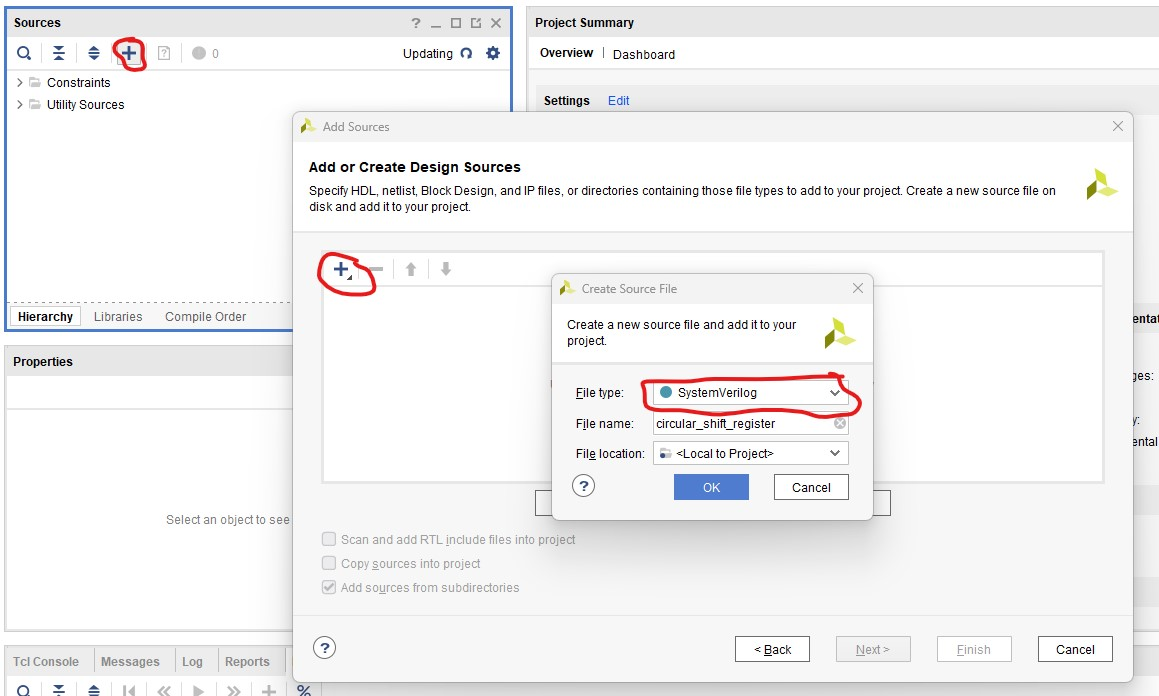
\includegraphics[width=9cm]{Images/CreateFile/create_system_verilog_file.jpg}
    \caption{Create a System Verilog File}
    \label{fig:enter-label}
\end{figure}
\begin{itemize}
    \item Select the Plus in the Sources Window
    \item Select "Add or create design sources"
    \item Select the Plus in the wizard window
    \item Select "Create File..."
    \item Give the file a name: \textit{circular\_shift\_register}. And be sure to select System Verilog.
    \item Select Finish
\end{itemize}
\begin{figure}[H]
    \centering
    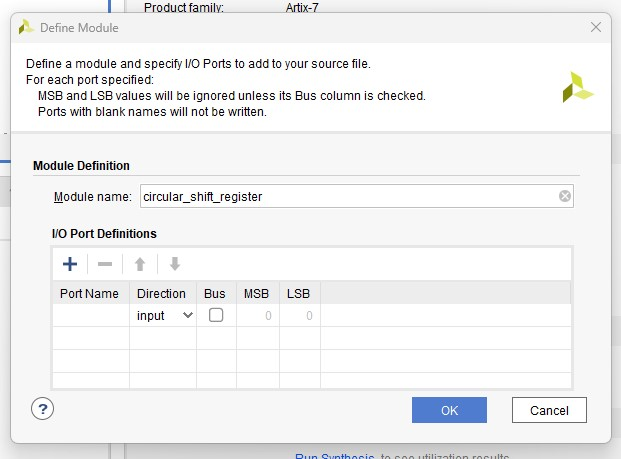
\includegraphics[width=9cm]{Images/CreateFile/DefineModule.jpg}
    \caption{Define Module Window}
    \label{fig:enter-label}
\end{figure}
The define module window will pop up. This defines the input and output ports for the module being designed. Add the ports to the window to produce the following ports. Select bus and adjust MSB to create ports of more than one bit.
\begin{itemize}
    \item Create an input port named clk,
    \item Another Input port named rst\_n,
    \item And finally an output port named reg\_out, make it a bus and make it 128 bits wide (This means the MSB is 127, not 128!)
\end{itemize}
Opening up your module you should see the following:
\begin{verbatim}
    module circular_shift_register(
    input clk,
    input rst_n,
    output [127:0] reg_out
    );
endmodule
\end{verbatim}
The very long register as it is created here will be difficult to work with. Therefore we want to change it to a packed array of 16 8-bit registers. To this end change the register out to be:
\begin{verbatim}
    output logic [7:0] reg_out[15:0]
\end{verbatim}
Now with that setup we can start by declaring the register internally.
\begin{verbatim}
    logic [7:0] circ_reg [15:0];
    assign reg_out = circ_reg;
\end{verbatim}
While we could work directly with the output register instead of having this internal declaration it can be good practice to split it like this as in larger designs it can allow for additional layers of abstraction or for hiding internal states when working with more complicated designs.

\begin{lstlisting}

// Always block triggered by a positive edge of the clock
always_ff @(posedge clk) begin
    if (!rst_n) begin
        // Reset the register array to the initial state
        circ_reg <= ??
|\colorbox{magenta!30}{// Assign appropriate reset values to every element of the circular shift register}|
    end else begin
        // Circularly shift the register array
        circ_reg <= ??
|\colorbox{magenta!30}{// Create the circular shifting register behavior}|
    end
end
\end{lstlisting}

You'll need to create a synchronous reset which will set the value of each 8-bit register in circ\_reg, then on every clock cycle you'll need to create a shift register behavior where the last value in the register becomes the first. Once you believe you have this you'll need to create a new file for the test bench.\\

This module is simple enough that you can practically test every possible state by declaring the device under test, resetting the registers to bring them into known states, and running through the clock 16 times to cycle through all possible values. You can also be much more creative with the test bench if you so choose.

\begin{lstlisting}
module tb_circular_shift_register;

    // Parameters
    parameter WIDTH = 8;
    parameter SIZE = 16;

    // Clock and reset signals
    logic clk;
    logic rst_n;

    // Output array for observing the register state
    logic [WIDTH-1:0] reg_out[SIZE-1:0];

    // Instantiate DUT
    circular_shift_register u_circular_shift_register (
        .clk(clk),
        .rst_n(rst_n),
        .reg_out(reg_out)
    );

    // Clock generation
    always begin
        #5 clk = ~clk; // 10 time unit period
    end

    // Testbench stimulus
    initial begin
        // Initialize signals
        clk = 0;
        rst_n = 0;
        
        // Apply reset
        #10 rst_n = 1;

        // Loop through 16 cycles and print the register state
        repeat (SIZE) begin
            #10; // Wait for one clock cycle
            $display("Register State:");
            $display("reg_out[0] = %h",reg_out[0]) ;
            ... ...
        end

        // Finish the simulation
        $finish;
    end

endmodule
\end{lstlisting}
You can use this to test your circular shift register. You will potentially want to add some additional code to improve the test bench. You can add checks to confirm that it is indeed circling, or you can manually observe the behavior in the waveform window. 
\subsubsection{Create Top Level}

With the test bench and this module complete you have the minimum needed number of lower level cells. You could decide to make a specialized cell for clock division, or you can reuse the PWM module with appropriate values to produce a slow clock. You need this slower clock to drive your circular shift register so that you can visualize the patterns being created. You can use the provided PWM test bench to find a good maximum value, and duty cycle through trial and error or deliberate calculation. \\
\vspace{0.5cm}
For the top level:
\begin{itemize}
    \item Instantiate 16 copies of the PWM module. Hook one PWM module up to each LED output. 
    \item Instantiate 1 copy of your circular shift register. Hook each PWM duty cycle up to one of the output registers. 
    \item Instantiate either an appropriately configured PWM module, or a dedicated clock divider to produce a slow clock for the circular shift register. 
    \item Modify the provided top level test bench and produce the needed text file to run through the python web application to verify your results visually. 
\end{itemize}
Extend the LED Output on the top module.
\begin{verbatim}
    output reg [15:0] led
\end{verbatim}
Declare 16 copies of the PWM Module
\begin{verbatim}
    pwm_module #(
        .bit_width(bit_width)
    ) pwm_unit (
        .clk(clk),
        .rst_n(rst_n),
        .duty(duty[i]),
        .max_value(8'd255),
        .pwm_out(pwm_out[i])
    );
\end{verbatim}
For these modules we are going to want a bit width of 8 bits to match with the circular shift register we created, and then we are going to set our maximum value to 255. duty[i] is going to be outputs from the circular shift register and will be 0 to 15. We will need to declare the associated logic to hook up from the pwm modules to the circular shift register. Finally pwm\_out is going to be directed towards the 16 led outputs. \\

Let's declare the variables to hook everything together.
\begin{verbatim}
    logic rst_n;
    logic [7:0] duty [15:0];
    logic [15:0] pwm_out;
    // Output of the circular shift register
    logic [7:0] reg_out [15:0]; 
    // Reduced clock signal for the circular shift register
    logic clk_reduced; 
\end{verbatim}

You can see here I have declared rst\_n. This is because I have added this line to the top module.
\begin{verbatim}
    assign rst_n = ~reset;
\end{verbatim}
This is technically breaking the rule of no logic on the top level of a design. But this can be considered the absolute most that is acceptable, even if it is frowned upon. If you want to adhere to absolute best practices, create an additional module which will take a reset input, and deliver rst, and rst\_n outputs. These outputs may be generated through either combinational or sequential logic. In larger designs appropriate handling of reset can become a significant challenge. 

\begin{verbatim}
    circular_shift_register csr (
        .clk(clk_reduced),
        .rst_n(rst_n),
        .reg_out(reg_out)
    );
\end{verbatim}

Declare your circular shift register. You'll notice that I'm feeding it a reduced clock speed. If cycling at the 100MHz clock cycle it would loop around every 160ns, even if the pwm module were running fast enough to reflect this it is far too fast for our eyes to see. Next you'll want to declare an additional PWM module to generate your output values. 

\begin{verbatim}
        pwm_module #(
        .bit_width(?) 
    ) clk_reducer (
        .clk(clk),
        .rst_n(rst_n),
        .duty(?), 
        .max_value(?),
        .pwm_out(clk_reduced)
    );
\end{verbatim}

Find appropriate values for duty, max\_value, and bit\_width to create a visible cycling of the led brightness.\\
\vspace{1cm}
Lastly \textbf{remember} to add appropriate assigns to connect the circular shift register to the pwm modules, and the pwm outputs to the leds. With this complete create a new top level test bench to verify the behavior. 

\subsubsection{Top Level Test bench}
You can reuse the old top level test bench. With a few minor changes. 
\begin{itemize}
    \item Remove the switch adjusting behavior and simply wait a long period of time after the reset is complete.
    \item Modify the print to file function call to pass all the led values. Removing the zeros and replacing them with the led values. \begin{verbatim}
        print_leds_to_file({led,15'b000000000000000}, file_descriptor);
    \end{verbatim}
\end{itemize}

Run your simulation again, this will take 5 - 20 minutes. Afterwards your led.txt will contain lines like this:
\begin{verbatim}
    0.0000150000 0000000000000000
    0.0000450000 1111111111111111
    0.0000550000 0000011111111000
    0.0002150000 0000001111110000
    0.0003750000 0000000111100000
    0.0006950000 0000000011000000
\end{verbatim}
The timing will be different and will shift as you progress through the very long file. You can then produce a video representation to confirm you have a good led pattern using the same online tool as for the original design. 

\begin{figure}[H]
    \centering
    
\includegraphics[height=1cm]{Images/ProvidedPWM/FinalOutput.jpg}
    \caption{Generated Video Output}
    \label{fig:enter-label}
\end{figure}

\section{Marking}
Your marks are split evenly between your code and the explainer video.\\
\begin{itemize}
    \item Include all the required files for your design and test benches. This means that all the System Verilog Files are present even if they are unmodified. Also be sure to include the associated constraints file.
    \item Ensure the provided code produces an led pattern at a speed which is clear at human time-scales. 
    \item Include a design report file. This should include your timing constraints and a calculation of the maximum operating frequency for your design. It also needs to include a screenshot of your RTL view after making the modifications. Your report should have a cover page containing your Name, Student ID, Lab Section, and Lab Title. 
    \item \textbf{Create a timing diagram showing pulse width modulation and explaining why it can be used to produce a dimming effect with LEDs. Include this in your design report alongside the other material}. Feel free to use tools like  \url{https://wavedrom.com/} to produce your timing diagrams. If using one of these tools make sure to include the text used to generate the waveform diagram. 
    \item Record a short 1-3 minute video explaining what you have done. Look at each segment of your code and explain approximately how it is working. 
\end{itemize}

\vspace{0.5cm}
Provide a video of you walking through each section of your code and explaining your reasoning. Your video should be no more than 4 minutes long. Ensure that you are clearly audible through the video. 
\section{Playing with your FPGA}
Learning through play is generally agreed to be the best approach to learning regardless of your age. To help you prepare for your midterm I suggest writing additional HDL code. In this lab you created a fun pattern on the LED output of the Basys 3. To go further add an option to change the direction of the wave by pressing a button, or disable the LED's by flipping a switch. If you do this, you will be able to potentially reuse this module in Lab 3 or 4 to make your design more visually impressive.
\end{document}
